\subsection{\textit{k}-Nearest Neighbors (KNN)}

\textit{k}-Nearest Neighbors (KNN) merupakan algoritma pembelajaran mesin non-parametrik
berbasis instans (\textit{instance-based learning}) yang tergolong sebagai \textit{lazy learner}.
KNN tidak membentuk fungsi pemetaan eksplisit selama tahap pelatihan, melainkan menyimpan
seluruh sampel data latih dan menunda seluruh proses komputasi hingga tahap inferensi.
Untuk mengklasifikasikan sampel kueri $x \in \mathbf{R}^d$, KNN mengukur jarak antara $x$
dengan seluruh data latih, memilih $k$ tetangga terdekat $\mathcal{N}_k(x)$, lalu
menentukan kelas prediksi berdasarkan agregasi label dari tetangga-tetangga tersebut.

Jarak antara dua titik data $x, z \in \mathbf{R}^d$ dihitung menggunakan metrik jarak
Minkowski tingkat $p$:
\[
D(x, z) = \left( \sum_{j=1}^d |x_j - z_j|^p \right)^{\frac{1}{p}} .
\]
Kasus khusus dari metrik ini mencakup jarak Manhattan ($p=1$) dan jarak Euclidean ($p=2$).
Untuk fitur berskala biner atau kategorikal, jarak Hamming ternormalisasi didefinisikan sebagai
$D_{\text{Hamming}}(x, z) = \frac{1}{d} \sum_{j=1}^d [x_j \neq z_j]$, dengan $[P]$ bernilai 1 jika kondisi $P$ benar dan 0 jika sebaliknya (notasi Iverson).

Pada skema penentuan label mayoritas (\textit{majority voting}), prediksi kelas ditentukan
melalui pembobotan seragam (\textit{uniform}):
\[
\hat{y} = \arg\max_{c \in \mathcal{C}} \sum_{i \in \mathcal{N}_k(x)} [y_i = c] .
\]
Namun, pembobotan seragam rentan terhadap bias jika kerapatan tetangga tidak merata.
Untuk mengatasi hal ini, diterapkan pembobotan jarak terbalik (\textit{inverted distance weighting}),
di mana tetangga yang berada lebih dekat memberikan kontribusi suara lebih besar:
\[
w_i = \frac{1}{D(x, x_i) + \epsilon}, \qquad
\hat{y} = \arg\max_{c \in \mathcal{C}} \sum_{i \in \mathcal{N}_k(x)} w_i \cdot [y_i = c] ,
\]
dengan konstanta penghalus $\epsilon = 10^{-5}$ guna mencegah pembagian dengan nol.
Estimasi probabilitas posterior kelas dihitung melalui normalisasi skor bobot tetangga:
\[
P(y = c \mid x) = \frac{\sum_{i \in \mathcal{N}_k(x)} w_i \cdot [y_i = c]}{\sum_{i \in \mathcal{N}_k(x)} w_i} .
\]
Pada klasifikasi biner dataset pembatalan reservasi hotel (\texttt{is\_canceled}), keputusan akhir
dapat dikalibrasikan menggunakan ambang batas probabilitas $\theta$: sampel diprediksi positif ($1$)
jika $P(y=1 \mid x) \ge \theta$, dan negatif ($0$) jika sebaliknya.

\subsubsection{Implementasi}

Implementasi KNN dari nol (\textit{from scratch}) diorganisasi secara modular pada berkas
\texttt{src/models/knn.py} serta dieksplorasi secara interaktif pada \texttt{notebooks/knn.ipynb}.
Kelas utama \texttt{KNN} mewarisi antarmuka \texttt{BaseModel} dengan tiga fitur arsitektur utama:

\begin{itemize}
  \item \textbf{Komputasi Jarak Berbasis \textit{Batch} (\texttt{\_distances})}:
        Menghitung matriks jarak $N_{\text{batch}} \times N_{\text{train}}$ secara terkotak-kotak
        (\textit{chunked batch}, bawaan $\text{batch\_size} = 256$) memanfaatkan \textit{broadcasting}
        NumPy. Strategi ini secara drastis mencegah lonjakan memori (\textit{Out-of-Memory}) yang
        rentan terjadi jika matriks jarak penuh dialokasikan secara simultan pada data berukuran puluhan ribu.
  \item \textbf{Seleksi Tetangga Cepat (\texttt{np.argpartition})}:
        Alih-alih melakukan pengurutan penuh $O(N \log N)$ dengan \texttt{argsort}, algoritma
        menggunakan partisi parsial \texttt{np.argpartition} yang beroperasi dalam kompleksitas waktu
        linear rata-rata $O(N)$ untuk mengambil $k$ indeks tetangga terdekat.
  \item \textbf{Dukungan Pembobotan dan Kalibrasi Ambang}:
        Mendukung skema bobot \texttt{"uniform"} maupun \texttt{"inverted"}, serta metode
        \texttt{predict\_proba} untuk penyesuaian ambang klasifikasi yang adaptif terhadap ketidakseimbangan kelas.
\end{itemize}

Cuplikan fungsi utama komputasi jarak dan inferensi disajikan pada Listing~\ref{lst:knn-core}.

\begin{lstlisting}[caption={Komputasi jarak berbasis batch dan inferensi pada kelas \texttt{KNN}.},label={lst:knn-core}]
def _distances(self, Xb: np.ndarray) -> np.ndarray:
    n_feat = self.X_train_.shape[1]
    D = np.zeros((Xb.shape[0], self.X_train_.shape[0]))
    if self.metric == "hamming":
        for j in range(n_feat):
            D += Xb[:, j][:, None] != self.X_train_[:, j][None, :]
        return D / n_feat
    for j in range(n_feat):
        D += np.abs(Xb[:, j][:, None] - self.X_train_[:, j][None, :]) ** self.p
    return D ** (1 / self.p)

def predict(self, X: np.ndarray) -> np.ndarray:
    preds = []
    for start in range(0, X.shape[0], self.batch_size):
        Xb = X[start : start + self.batch_size]
        D = self._distances(Xb)
        idx = np.argpartition(D, self.k - 1, axis=1)[:, : self.k]
        labels = self.y_train_[idx]
        if self.weights == "inverted":
            k_dist = np.take_along_axis(D, idx, axis=1)
            w = 1.0 / (k_dist + 1e-5)
            scores = np.stack([(w * (labels == c)).sum(axis=1) for c in self.classes_], axis=1)
            preds.append(self.classes_[np.argmax(scores, axis=1)])
        else:
            counts = np.stack([(labels == c).sum(axis=1) for c in self.classes_], axis=1)
            preds.append(self.classes_[np.argmax(counts, axis=1)])
    return np.concatenate(preds)
\end{lstlisting}

\paragraph{Prapemrosesan Data untuk KNN.}
Model KNN memanfaatkan masukan data yang diproses melalui pipeline pada Subbab~\ref{subsec:preprocessing},
yaitu penskalaan standar (\texttt{StandardScaler}), seleksi 15 fitur terbaik (\texttt{SelectKBest}),
dan reduksi dimensi menjadi 9 komponen utama (PCA). Khusus pada model KNN, pelatihan dilakukan
secara eksklusif hanya pada baris data asli (\texttt{fit\_orig\_only}) tanpa mengikutsertakan sampel
sintetis SMOTE guna menghindari distorsi batas lokal tetangga, dengan penanganan ketidakseimbangan
kelas dialihkan pada kalibrasi ambang batas probabilitas (\texttt{prob\_thres} $\approx 0{,}45$).

\subsubsection{Hasil dan Perbandingan dengan scikit-learn}

Evaluasi komparatif dilakukan secara terkontrol antara implementasi KNN \textit{from scratch}
dengan \texttt{sklearn.neighbors.KNeighborsClassifier}. Pengujian menggunakan data validasi
asli yang identik, meliputi variasi parameter jumlah tetangga $k \in \{3, 5, 7\}$ serta skema
pembobotan suara (\textit{uniform} vs \textit{inverted distance}). Hasil kuantitatif dirangkum
pada Tabel~\ref{tab:knn-comparison}.

\begin{table}[htbp]
  \centering
  \caption{Perbandingan performa klasifikasi dan efisiensi komputasi antara KNN \textit{from scratch}
  dan \texttt{scikit-learn} pada subset validasi terstratifikasi (4.000 data latih, 1.000 data validasi).}
  \label{tab:knn-comparison}
  \footnotesize
  \begin{tabular}{lllcccccc}
    \toprule
    $k$ & Bobot & Model & Akurasi & Macro-F1 & F1 Kelas 1 & Waktu Latih & Waktu Inferensi & Kesepakatan \\
    \midrule
    3 & Uniform  & Scratch & 0,7840 & 0,7489 & 0,6550 & 0,12 ms & 600,79 ms & \textbf{100,00\%} \\
      &          & sklearn & 0,7840 & 0,7489 & 0,6550 & 32,42 ms & 0,04 ms  & \\
    \midrule
    3 & Inverted & Scratch & 0,7950 & 0,7631 & 0,6761 & 0,15 ms & 667,60 ms & \textbf{100,00\%} \\
      &          & sklearn & 0,7950 & 0,7631 & 0,6761 & 11,24 ms & 0,04 ms  & \\
    \midrule
    5 & Uniform  & Scratch & 0,7920 & 0,7556 & 0,6612 & 0,20 ms & 642,36 ms & \textbf{100,00\%} \\
      &          & sklearn & 0,7920 & 0,7556 & 0,6612 & 9,46 ms  & 0,04 ms  & \\
    \midrule
    5 & Inverted & Scratch & 0,8020 & 0,7694 & 0,6827 & 0,09 ms & 661,47 ms & \textbf{100,00\%} \\
      &          & sklearn & 0,8020 & 0,7694 & 0,6827 & 9,92 ms  & 0,03 ms  & \\
    \midrule
    7 & Uniform  & Scratch & 0,8020 & 0,7669 & 0,6765 & 0,10 ms & 617,85 ms & \textbf{100,00\%} \\
      &          & sklearn & 0,8020 & 0,7669 & 0,6765 & 14,59 ms & 0,06 ms  & \\
    \midrule
    7 & Inverted & Scratch & 0,8070 & 0,7734 & 0,6862 & 0,14 ms & 625,71 ms & \textbf{100,00\%} \\
      &          & sklearn & 0,8070 & 0,7734 & 0,6862 & 16,74 ms & 0,05 ms  & \\
    \bottomrule
  \end{tabular}
\end{table}

Berdasarkan Tabel~\ref{tab:knn-comparison}, diperoleh beberapa temuan signifikan:
\begin{itemize}
  \item \textbf{Akurasi Matematis dan Kesepakatan Prediksi}:
        Pada seluruh konfigurasi parameter $k$ dan skema bobot yang diuji, metrik Akurasi,
        Macro-F1, dan F1-Score kelas positif model \textit{from scratch} sama persis hingga empat digit
        desimal dengan scikit-learn. Tingkat kesepakatan prediksi (\textit{prediction agreement}) mencapai
        \textbf{100,00\%}, membuktikan bahwa logika partisi tetangga dan formula pembobotan jarak
        yang diimplementasikan secara mandiri telah valid dan sejalan dengan standar pustaka industri.
  \item \textbf{Karakteristik Efisiensi Waktu}:
        Tahap pelatihan (\textit{fit}) model \textit{from scratch} berlangsung sangat cepat ($< 0{,}2$ ms)
        karena murni menyimpan matriks fitur ke dalam memori ($O(1)$). Sebaliknya, scikit-learn
        memerlukan waktu pelatihan berkisar 9--32 ms karena membangun struktur pohon indeks (\textit{KD-Tree} atau \textit{Ball-Tree}).
        Namun pada tahap inferensi, scikit-learn jauh lebih cepat karena pencarian tetangga terindeks pohon
        yang dioptimalkan dengan kompilasi Cython, sementara model \textit{from scratch} menghitung jarak
        secara \textit{brute-force batch} dalam interpreted Python/NumPy.
  \item \textbf{Keunggulan Skema Pembobotan Inverted}:
        Pada setiap nilai $k$, pembobotan \textit{inverted distance} secara konsisten mengungguli
        pembobotan \textit{uniform} dengan selisih peningkatan Macro-F1 sebesar $0{,}007$ hingga $0{,}014$.
        Hal ini menegaskan bahwa memberikan bobot proporsional terhadap kedekatan geometris efektif
        mereduksi pengaruh tetangga yang berada jauh atau berada di wilayah batas keputusan.
\end{itemize}

\begin{figure}[htbp]
  \centering
  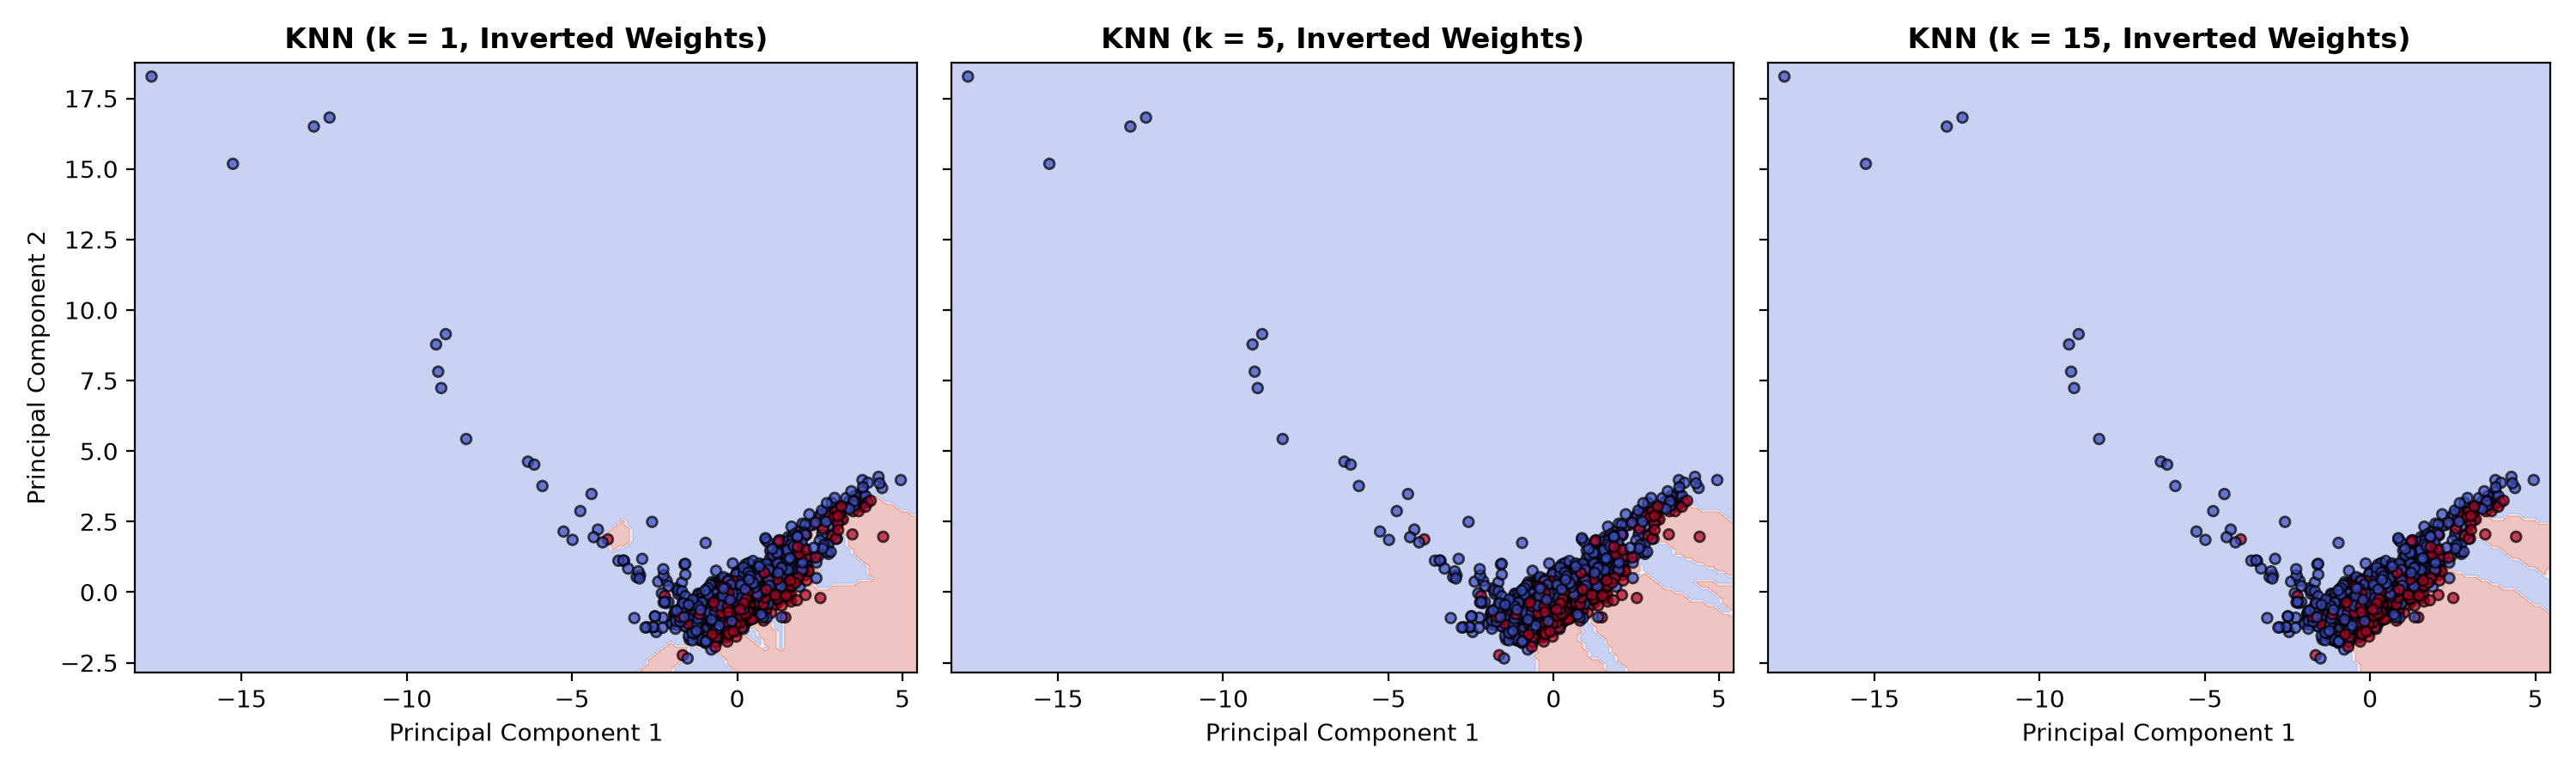
\includegraphics[width=0.95\linewidth]{assets/knn/knn-decision-boundary.png}
  \caption{Visualisasi batas keputusan KNN (\textit{inverted weights}) pada proyeksi dua komponen
  utama pertama untuk variasi nilai $k \in \{1, 5, 15\}$.}
  \label{fig:knn-boundary}
\end{figure}

Visualisasi pada Gambar~\ref{fig:knn-boundary} memperlihatkan dampak pemilihan nilai $k$ terhadap bentuk batas keputusan:
\begin{itemize}
  \item Pada $k=1$, batas keputusan sangat terfragmentasi dan membentuk pulau-pulau kecil di sekitar
        titik pencilan (\textit{overfitting}).
  \item Pada $k=5$, batas keputusan menjadi jauh lebih halus dan kontur pemisah antarkelas terlihat wajar,
        mencapai keseimbangan optimal antara \textit{bias} dan \textit{variance}.
  \item Pada $k=15$, batas keputusan menjadi terlalu menyederhanakan sebaran lokal (\textit{underfitting}),
        sehingga titik-titik minoritas di area perbatasan cenderung terabaikan.
\end{itemize}

\paragraph{Evaluasi Validasi Silang dan Matriks Konfusi.}
Pada pengujian \textit{Stratified 5-Fold Cross Validation} terhadap data latih penuh (27.373 baris)
menggunakan konfigurasi optimal ($k=5$, metrik Euclidean, \textit{inverted weights}, dan ambang
probabilitas $\theta = 0{,}45$), diperoleh rata-rata akurasi sebesar \textbf{0,8395} dan rata-rata
Macro-F1 sebesar \textbf{0,8395} ($\pm 0{,}0032$).

\begin{figure}[htbp]
  \centering
  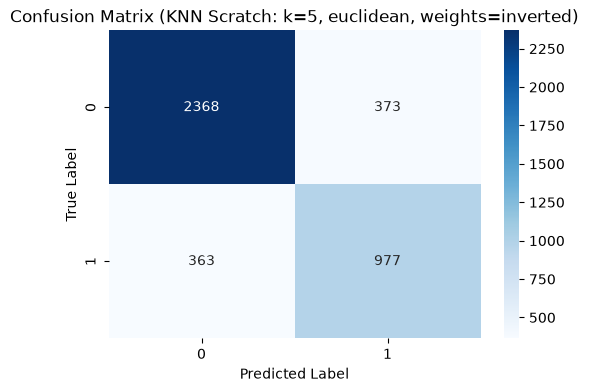
\includegraphics[width=0.48\linewidth]{assets/knn/knn-confusion-matrix.png}
  \caption{Matriks konfusi model KNN final ($k=5$, \textit{inverted weights}, ambang batas probabilitas $\theta = 0{,}45$)
  pada himpunan validasi data asli.}
  \label{fig:knn-cm}
\end{figure}

Matriks konfusi pada Gambar~\ref{fig:knn-cm} menunjukkan bahwa model berhasil mendeteksi pembatalan
(kelas positif 1) secara seimbang dengan \textit{recall} $73\%$ dan \textit{precision} $72\%$,
sementara kelas non-batal (kelas 0) diprediksi dengan presisi $87\%$ dan \textit{recall} $86\%$.
Penyetelan ambang batas pada $\theta = 0{,}45$ secara efektif meningkatkan sensitivitas terhadap pembatalan
tanpa mengorbankan akurasi global secara berlebihan.

\paragraph{Submisi Akhir.}
Model KNN final yang dilatih pada seluruh data latih asli menghasilkan berkas submisi
\texttt{submission\_knn.csv} (6.844 baris data uji). Distribusi hasil prediksi terdiri atas 4.841 sampel
kelas 0 ($70{,}74\%$) dan 2.003 sampel kelas 1 ($29{,}26\%$). Proporsi ini sangat selaras dengan rasio
alami kelas pada data latih asli ($32{,}77\%$ pembatalan), mengonfirmasi bahwa model tidak mengalami bias
ekstrem dan memiliki kemampuan generalisasi yang stabil.
